\documentclass[11pt]{article}
\usepackage{fontspec}
\usepackage{amsmath}
\usepackage{tikz}
\usetikzlibrary{arrows.meta,calc}
\usepackage{graphicx}
\usepackage{geometry}
\geometry{paperwidth=18cm, paperheight=22cm, margin=7mm}
\setmainfont{texgyrepagella-regular.otf}
\setsansfont{texgyreheros-regular.otf}
\pagestyle{empty}

\begin{document}
\noindent{\sffamily Reference}\\[1mm]
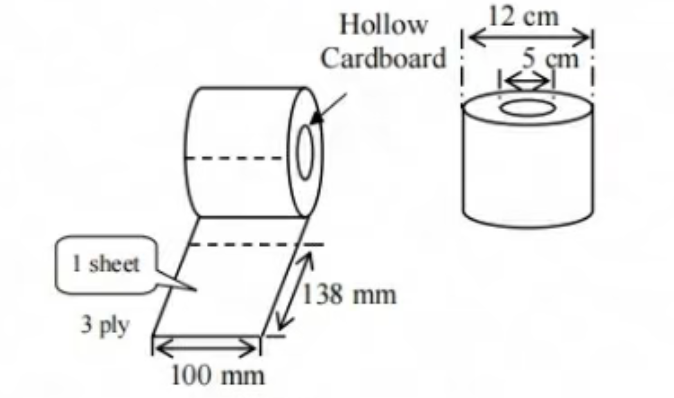
\includegraphics[width=0.88\textwidth]{../build/q15-user-ref.png}

\vspace{5mm}
\noindent{\sffamily TikZ}\\[1mm]
\begin{center}
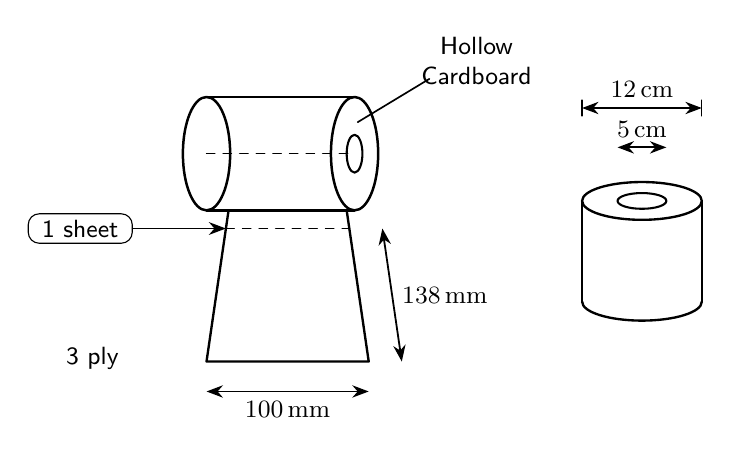
\begin{tikzpicture}[>=Stealth, line cap=round, line join=round, font=\sffamily\small]
  % ===== Left: 3-D horizontal roll =====
  \coordinate (R) at (2.20,3.55);
  \def\rx{0.30}
  \def\ry{0.72}
  \def\len{1.88}
  \coordinate (L) at ($(R)+(-\len,0)$);

  \fill[white]
    ($(L)+(0,-\ry)$) -- ($(R)+(0,-\ry)$)
    -- ($(R)+(0,\ry)$) -- ($(L)+(0,\ry)$) -- cycle;
  \draw[line width=0.9pt] ($(L)+(0,\ry)$) -- ($(R)+(0,\ry)$);
  \draw[line width=0.9pt] ($(L)+(0,-\ry)$) -- ($(R)+(0,-\ry)$);
  \filldraw[fill=white, draw=black, line width=0.9pt]
    (L) ellipse[x radius=\rx, y radius=\ry];
  \filldraw[fill=white, draw=black, line width=0.9pt]
    (R) ellipse[x radius=\rx, y radius=\ry];
  \filldraw[fill=white, draw=black, line width=0.75pt]
    (R) ellipse[x radius=0.10, y radius=0.24];
  \draw[dashed, line width=0.55pt] (L) -- (R);

  \node[align=center] (hc) at ($(R)+(1.55,1.18)$) {Hollow\\Cardboard};
  \draw[line width=0.6pt] ($(R)+(0.95,0.95)$) -- ($(R)+(0.04,0.40)$);

  % Mild trapezoid, dashed "1 sheet" line just under the roll
  \coordinate (STL) at ($(L)+(0.28,-\ry)$);
  \coordinate (STR) at ($(R)+(-0.10,-\ry)$);
  \coordinate (SBL) at ($(STL)+(-0.28,-1.92)$);
  \coordinate (SBR) at ($(STR)+(0.28,-1.92)$);
  \draw[line width=0.85pt] (STL) -- (SBL) -- (SBR) -- (STR);
  \coordinate (SDL) at ($(SBL)!0.88!(STL)$);
  \coordinate (SDR) at ($(SBR)!0.88!(STR)$);
  \draw[dashed, line width=0.55pt] (SDL) -- (SDR);

  \node[draw, rounded corners=4pt, inner xsep=5pt, inner ysep=2.2pt, fill=white] (onesheet)
    at ($(SDL)+(-1.85,0)$) {1 sheet};
  \draw[->, line width=0.7pt] (onesheet.east) -- (SDL);
  \node (threeply) at ($(SBL)+(-1.45,0.04)$) {3 ply};

  % 100 mm: width of the bottom edge
  \draw[<->, line width=0.65pt]
    ([yshift=-3.8mm]SBL) -- ([yshift=-3.8mm]SBR)
    node[midway, below] {\(100\,\mathrm{mm}\)};
  % 138 mm: from the dashed line DOWN to the bottom of the sheet
  \draw[<->, line width=0.65pt]
    ([xshift=4.2mm]SDR) -- ([xshift=4.2mm]SBR)
    node[midway, right] {\(138\,\mathrm{mm}\)};

  % ===== Right: upright roll (oblique, hidden rim dashed) =====
  \coordinate (U) at (5.85,2.95);
  \def\urx{0.76}
  \def\ury{0.24}
  \def\uh{1.28}
  \def\irx{0.31}

  \draw[line width=0.85pt] ($(U)+(-\urx,0)$) -- ($(U)+(-\urx,-\uh)$);
  \draw[line width=0.85pt] ($(U)+(\urx,0)$) -- ($(U)+(\urx,-\uh)$);
  \draw[line width=0.85pt]
    ($(U)+(-\urx,-\uh)$) arc[start angle=180,end angle=360,x radius=\urx,y radius=\ury];
  \filldraw[fill=white, draw=black, line width=0.85pt]
    (U) ellipse[x radius=\urx, y radius=\ury];
  \filldraw[fill=white, draw=black, line width=0.75pt]
    (U) ellipse[x radius=\irx, y radius=0.10];

  \draw[<->, line width=0.65pt]
    ($(U)+(-\urx,1.18)$) -- ($(U)+(\urx,1.18)$)
    node[midway, above] {\(12\,\mathrm{cm}\)};
  \draw[line width=0.5pt] ($(U)+(-\urx,1.08)$) -- ($(U)+(-\urx,1.28)$);
  \draw[line width=0.5pt] ($(U)+(\urx,1.08)$) -- ($(U)+(\urx,1.28)$);
  \draw[<->, line width=0.65pt]
    ($(U)+(-\irx,0.68)$) -- ($(U)+(\irx,0.68)$)
    node[midway, above] {\(5\,\mathrm{cm}\)};
\end{tikzpicture}
\end{center}
\end{document}
